% This example An LaTeX document showing how to use the l3proj class to
% write your report. Use pdflatex and bibtex to process the file, creating 
% a PDF file as output (there is no need to use dvips when using pdflatex).

% Modified 

\documentclass{l3proj}
\usepackage{datetime}
\usepackage{graphicx}

\begin{document}
\title{Algorithm Animator}
\author{Arthur Bigeard \\
		Alexander Ferguson \\
		Andrew Gibson \\
		Gediminas Leikus \\
		Liam Bell}
\usdate
\date{\today}
\maketitle
\begin{abstract}

Algorithm Animator - a teaching and learning tool for both students and teachers. A piece of software, which animates algorithms and produces a visual representation of how they work.

Our project - an API approach using Java and TimingFramework to develop the Algorithm Animator. Due to the fact that it is an API approach, the user of the software is required to know programming and Java, in particular, in order to use it. Animation of 3 common data structures - Arrays, Linked Lists and Binary Trees. Ability to export the animations to images or export Array animations to Flash.

This is the user manual to handle our API.
\end{abstract}
\educationalconsent

\chapter{API}
Our API consists of 3 data structure you can animate:
\begin{itemize}
\item Arrays
\item Heaps
\item LinkedLists
\end{itemize}

To begin with the API you are provided a simple Main class with a few lines of required code to run the animation.

\begin{figure}
\begin{center}
\begin{verbatim}


import java.awt.Color;

import AnimatedDataStructure.AnimatedDataStructure;
import AnimatedLinkedList.AnimatedLinkedList;
import AnimatedArray.AnimatedArray;

import java.util.Random;

public class Main {
    
    private static AnimatedDataStructure anim; //Declare the AnimatedDataStructure you want
	//to animate here
    public static int time = 200;
    
	public static void main(String[] args) {
        anim.endAnimation();
	}
	
}

\end{verbatim}
\end{center}
\caption{The Main class code}
\label{fig:main}
\end{figure}

The first thing you will need to do is instanciate an Animation object of the data structure you want to animate. There are two constructors for
each animated data structure from which you can choose:
\begin{itemize}
\item The default constructor which only requires you to pass an array of data
\item The custom window size constructor which takes 3 parameters: the array of data, the window width and window height
\end{itemize}

Each data structure has different animation calls which you can use to create your animation steps within your algorithm.
Every structure support the following calls:
\begin{itemize}
\item swap: takes the indexes of two elements to swap and an optional int to specify the duration of the animation in milliseconds
\item setColor: takes the index of the element changing color and a Color ENUM value
\item setInfo: takes a parameter String to display as an animation information
\end{itemize}

The LinkedList supports the following additional calls:
\begin{itemize}
\item findAndRemove: Find and removes the elements equal to a String s in a parameter AnimatedLinkedList
\item addToHead : adds the integer value i at the head of the LinkedList
\end{itemize}

The Heap supports the following additional call:
\begin{itemize}
\item add : adds the integer value i to the heap; this function maintains the binary tree ordered structure
\end{itemize}

To animate your algorithm you have to inject the appropriate API calls into your code where you manipulate your data structure, or when you want
do some highlighting on elements. Here is a sample animation code for an array sorting algorithm:

\begin{figure}
\begin{center}
\begin{verbatim}


import java.awt.Color;

import AnimatedDataStructure.AnimatedDataStructure;
import AnimatedLinkedList.AnimatedLinkedList;
import AnimatedArray.AnimatedArray;

import java.util.Random;

public class Main {
    
    private static AnimatedArray anim;//We're creating an animation on an array,
    //hence using the AnimatedArray AnimatedDataStructure
    public static int time = 200;

    public static void main(String[] args) {
        int[] arr = {1,2,3,4,5,6,7,8,9,0,1,2,3,4};
        anim = new AnimatedArray(arr);
        int i, j,t=0;
        for(i = 0; i < arr.length; i++){
            for(j = 1; j < (arr.length-i); j++){
                anim.setColor(j, Color.RED, "");
                anim.setColor(j-1, Color.RED, "");
                if(arr[j-1] > arr[j]){
                    t = arr[j-1];
                    arr[j-1]=arr[j];
                    arr[j]=t;
                    anim.swap(j, j-1, "Swapping");
                }
                anim.setColor(j, Color.BLUE, "");
                anim.setColor(j-1, Color.BLUE, "");
            }
            anim.setColor(j-1, Color.DARK_GRAY, "Gray out an element that's in it's place already.");
        }
        anim.endAnimation();
    }
	
}

\end{verbatim}
\end{center}
\caption{An array sorting algorithm example: bubblesort}
\label{fig:animationAlgorithm}
\end{figure}



\chapter{User interface}

The user interface is very simple and only consists in a few explicitely named button.

\begin{figure}
\begin{center}
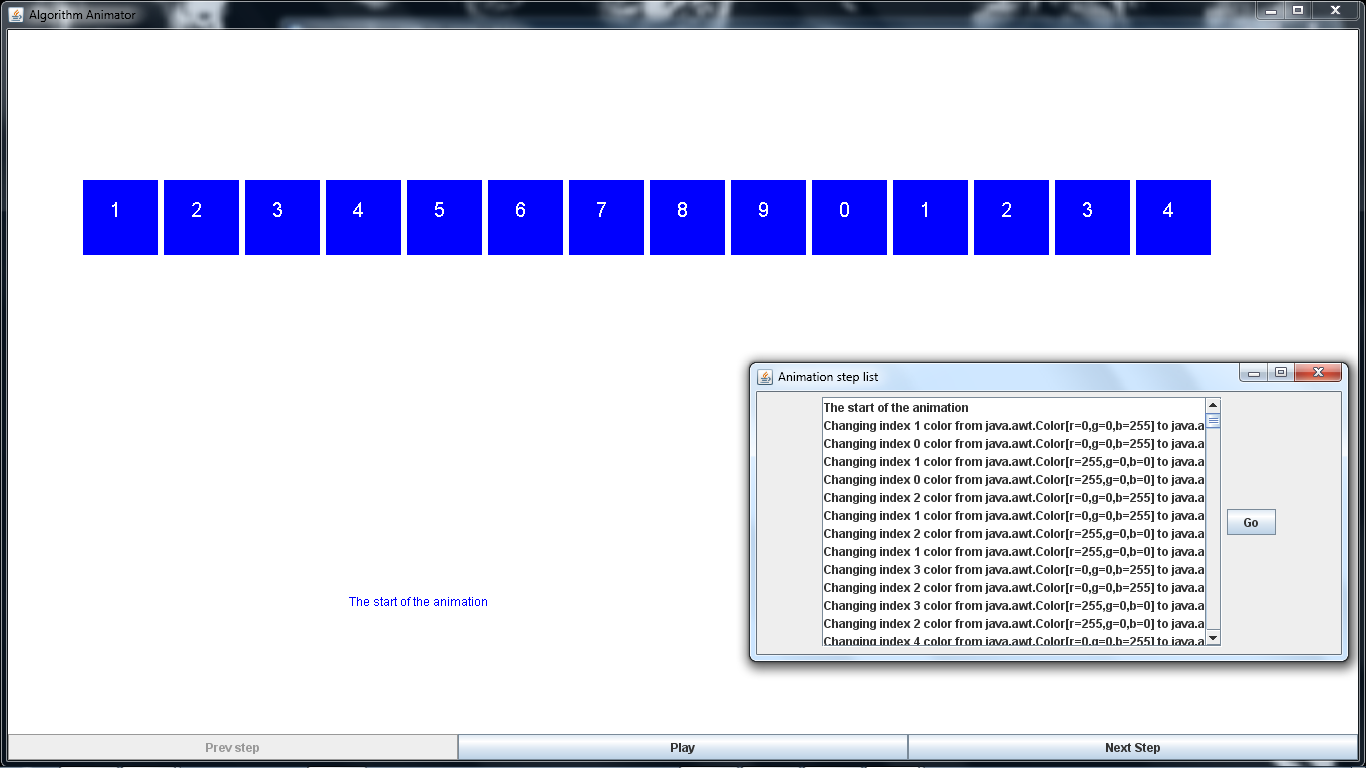
\includegraphics[width=\textwidth]{images/animationWindow.png}
\end{center}
\caption{TODO}
\label{fig:refactoring}
\end{figure}

When running the animation, you may use the middle Play/Pause button to run or stop the animation. There's two distinct animation
behaviours depending on wether the animation is running or not:
\begin{itemize}
\item If the animation is running, you won't be able to use the Prev/Next Step buttons
\item If the animation is paused, you may run it step by step using the Prev/Next Step buttons
\end{itemize}

Please take note that the Prev Step button will not animate the rollback to the previous step, it will simply restore the state of the animation to its previous state.
The Next Step Button on another hand will animate the change of state to the next step.

There is a second window opened with every animation running. It contains the entire list of animation steps, identified by their step description. When the animation is paused,
you may jump backward or forward in the animation by selecting the step you want to jump to and clicking the Go button. 
Please note that you may only use this feature while the animation is paused.